\documentclass{standalone}
\usepackage{tikz}
\usetikzlibrary{arrows.meta}

\begin{document}

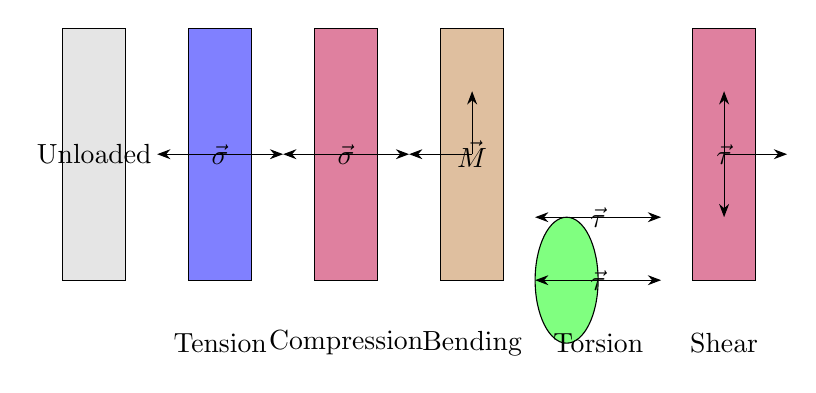
\begin{tikzpicture}[scale=0.8]
    % Unloaded
    \draw[fill=gray!20] (0,0) rectangle (1,4);
    \node at (0.5,2) {Unloaded};
    
    % Tension
    \draw[fill=blue!50] (2,0) -- (3,0) -- (3,4) -- (2,4) -- cycle;
    \draw[->,>=Stealth] (2.5,2) -- (3.5,2);
    \draw[->,>=Stealth] (2.5,2) -- (1.5,2);
    \node at (2.5,2) {$\vec{\sigma}$};
    \node at (2.5,-1) {Tension};
    
    % Compression
    \draw[fill=purple!50] (4,0) -- (5,0) -- (5,4) -- (4,4) -- cycle;
    \draw[->,>=Stealth] (4.5,2) -- (5.5,2);
    \draw[->,>=Stealth] (4.5,2) -- (3.5,2);
    \node at (4.5,2) {$\vec{\sigma}$};
    \node at (4.5,-1) {Compression};
    
    % Bending
    \draw[fill=brown!50] (6,0) -- (7,0) -- (7,4) -- (6,4) -- cycle;
    \draw[->,>=Stealth] (6.5,2) -- (5.5,2);
    \draw[->,>=Stealth] (6.5,2) -- (6.5,3);
    \node at (6.5,2) {$\vec{M}$};
    \node at (6.5,-1) {Bending};
    
    % Torsion
    \draw[fill=green!50] (8,0) ellipse (0.5cm and 1cm);
    \draw[->,>=Stealth] (8.5,0) -- (9.5,0);
    \draw[->,>=Stealth] (8.5,0) -- (7.5,0);
    \draw[->,>=Stealth] (8.5,1) -- (9.5,1);
    \draw[->,>=Stealth] (8.5,1) -- (7.5,1);
    \node at (8.5,0) {$\vec{\tau}$};
    \node at (8.5,1) {$\vec{\tau}$};
    \node at (8.5,-1) {Torsion};
    
    % Shear
    \draw[fill=purple!50] (10,0) -- (11,0) -- (11,4) -- (10,4) -- cycle;
    \draw[->,>=Stealth] (10.5,2) -- (11.5,2);
    \draw[->,>=Stealth] (10.5,2) -- (10.5,3);
    \draw[->,>=Stealth] (10.5,2) -- (10.5,1);
    \node at (10.5,2) {$\vec{\tau}$};
    \node at (10.5,-1) {Shear};
\end{tikzpicture}

\caption{Most common types of material deformations}
\label{fig:material_deformations}

\end{document}